\chapter{Solver nonogramów}
\thispagestyle{chapterBeginStyle}

    W tym rozdziale opisany jest rozwój solvera. Opisane są kolejne główne wersje solverów, zbadany
jest także wpływ zastosowanych heurystyk na wydajność w rozwiązywaniu wybranych łamigłówek.



\section{Wersje solverów}


\subsection{Solver całościowy}
    Solver całościowy jest najprostszym z solverów implementowanych w toku pisania aplikacji. Jego
implementacja opiera się na założeniu, że obrazek ukryty w łamigłówce jest ciągiem pustych i pełnych
pikseli. Solver sprawdza wszystkie możliwe kombinacje pól, aż do wykrycia rozwiązania, bądź stwierdzenia
jego braku. Wskazówki umieszczone obok planszy służą jedynie do walidacji rozwiązania, i nie są
wykorzystywane w trakcie rozwiązywania nonogramu.

\begin{figure}[!htb]
    \centering
    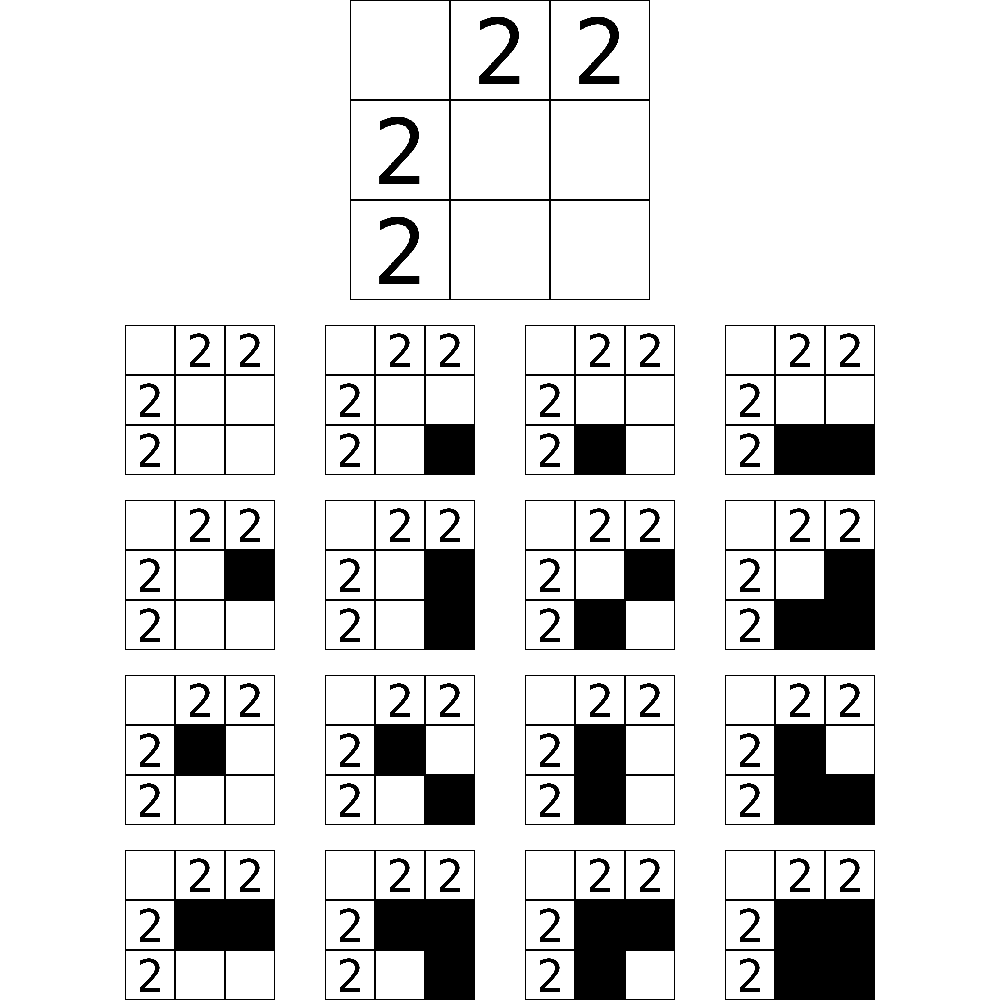
\includegraphics[width=0.5\textwidth]{images/all_solver_example.png}
    \caption{Solver całościowy sprawdza wszystkie możliwe układy planszy w celu znalezienia rozwiązania.}
\end{figure}

    Solver ten zaczyna od pustej planszy. Następnie, dla pierwszego pola wywoływana jest rekursyjna
metoda: jeśli indeks pola mieści się w zakresie planszy, to najpierw jego status ustawiany jest na
pusty, i następuje wywołanie metody dla nastepnego indeksu, a jeśli rozwiązanie nie zostanie znalezione,
to pole jest wypełniane i ponownie dochodzi do wywołania metody na następnym polu. Jeśli indeks
wykracza poza zakres planszy, to znaczy że wszystkie pola mają ustawiony status i wywoływana jest
metoda sprawdzająca poprawność rozwiązania, podobna do tej opisanej w \ref{alg:axisValidation}.
Jeśli solver zakończy działanie zwracając \texttt{true}, to w przekazanej mu macierzy pól 
(równoznaczne z listą wierszy) znajdzie się rozwiązanie łamigłówki.

\begin{pseudokod}[H]
    %\SetAlTitleFnt{small}
    \SetArgSty{normalfont}
    \SetKwFunction{Verify}{Verify}
    \KwIn{Lista wierszy $R$, indeks pola $i$, lista wskazówek wierszy $Hr$ i kolumn $Hc$, szerokość $w$ i wysokość $h$ planszy}
    \KwOut{Czy znaleziono rozwiązanie \texttt{true/false}}
    \If{$i \geq w \cdot h$}{
        \texttt{return} \Verify{$R$, $Hr$, $Hc$, $w$, $h$}\;
    }
    \Else{
        $iWiersza \leftarrow \lceil \frac{i}{w} \rceil$\;
        $iKolumny \leftarrow i\ mod\ w$\;
        $R[iWiersza][iKolumny] \leftarrow 0$\;
        \If{\texttt{SolverCałościowy}($R, i+1, Hr, Hc, w, h$)}{
            \texttt{return true}\;
        }
        $R[iWiersza][iKolumny] \leftarrow 1$\;
        \texttt{return SolverCałościowy}($R, i+1, Hr, Hc, w, h$)\;
    }
    \caption{SolverCałościowy}\label{alg:allSolver}
\end{pseudokod}

    Złożoność czasowa tego solvera jest bardzo duża. Procedura sprawdzająca poprawność rozwiązania
może zostać wywołana $2^{w*h}$ razy, czyli inaczej $2^n$, gdzie $n$ to ilość pól na planszy. 
Wynika to z faktu, że kazde kolejne pole wymaga sprawdzenia pól poprzednich, a samo może znajdować
się w dwóch stanach, więc podwaja ilość wywołań procedury sprawdzającej.


\subsection{Solver osiowy}
    W odróżnieniu od solvera całościowego, solver osiowy korzysta ze wskazówek przy szukaniu rozwiązań.
Opiera się on na fakcie, że każda linia (wiersz lub kolumna) może znajdować się w jednym z możliwych
stanów, których liczba nigdy nie dojdzie do $2^x$, gdzie $x$ jest długością linii. Sprawdzając
rozwiązanie w tym solverze, gwarantowana jest poprawność w jednej z osi, co dodatkowo znacząco skraca
czas szukania rozwiązania.

\begin{figure}[!htb]
    \centering
    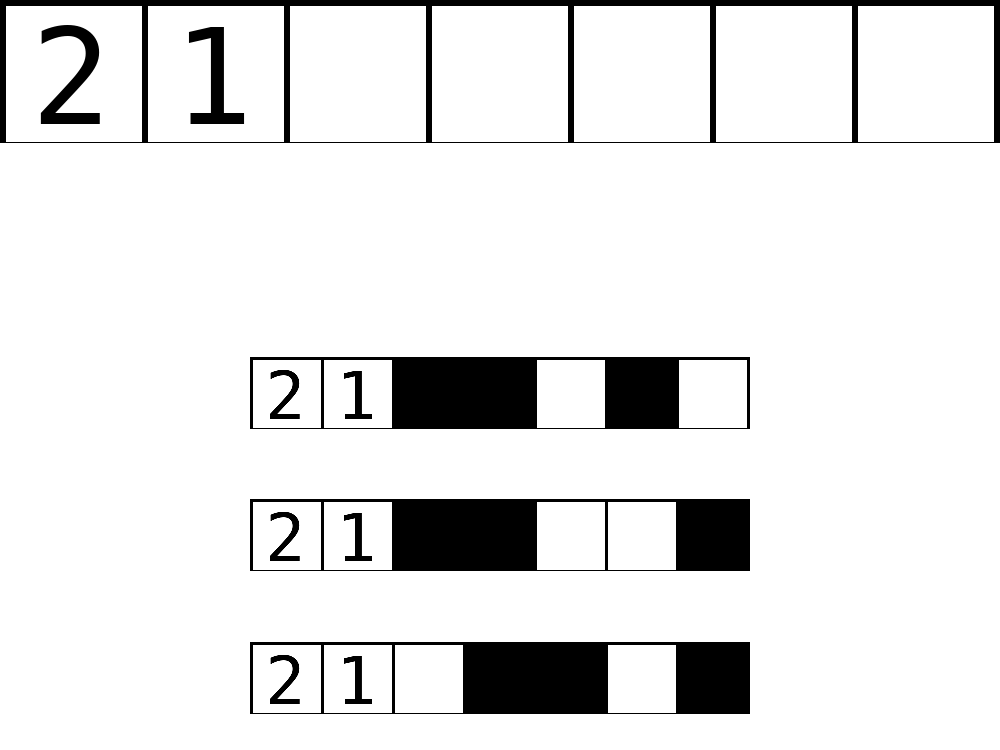
\includegraphics[width=0.5\textwidth]{images/axis_solver_example.png}
    \caption{Dla linii na grafice, solver osiowy spradza jedynie 3 stany. Dla tej samej linii,
solver całościowy sprawdziłby $2^5 = 32$ stany
    }
\end{figure}

    Solver zaczyna od pustej planszy. Przed rozpoczęciem rozwiązywania sprawdzana jest ilość wszystkich
kombinacji w danej osi (iloczyn możliwości każdej z linii), i wybierana jest oś z mniejszą liczbą
możliwości. Następnie generowane są kombinacje dla każdej z linii. Solver korzysta z rekursyjnej
metody, i ustawia pierwszą kombinację dla pierwszej linii. Następnie wywołuje metodę dla kolejnej linii,
aż do ostatniej, i wtedy weryfikuje rozwiązanie. Jeśli dla danego ustawienia w linii łamigłówka
nie ma rozwiązania, to solver przechodzi do kolejnego ustawienia i wywołuje metodę w kolejnej linii.

\begin{pseudokod}[H]
    %\SetAlTitleFnt{small}
    \SetArgSty{normalfont}
    \SetKwFunction{Verify}{Verify}
    \SetKwFunction{NalozKombinacje}{NalozKombinacje}
    \KwIn{Lista linii $L$, indeks linii $i$, lista wskazówek linii prostopadłych $H$, ilość linii $n$}
    \KwOut{Czy znaleziono rozwiązanie \texttt{true/false}}
    \If{$i = n$}{
        \texttt{return} \Verify{$L$, $H$, $n$}\;
    }
    \Else{
        $linia \leftarrow L[i]$\;
        \ForEach{$komb \in linia.kombinacje$}{
            \NalozKombinacje{$linia, komb$}\;
            \If{\texttt{SolverOsiowy}($L, i+1, H, n$)}{
                \texttt{return true}\;
            }
        }
        \texttt{return false}\;
    }
    \caption{SolverOsiowy}\label{alg:axisSolver}
\end{pseudokod}

    Dzięki eliminacji kombinacji sprzecznych ze wskazówkami w danej osi, procedura sprawdzania
poprawności rozwiązania jest wywoływana o wiele rzadziej niż w przypadku solvera całościowego.
O ile ilość kombinacji w linii przy rozpatrywaniu każdej komórki z osobna to $2^n$, gdzie $n$ to
długość linii, tak w przypadku rozważania poprawnych kombinacji dla linii jest ona zależna od
długości i zawartości wskazówki, i można ją ograniczyć z góry przez
${n + 1 - h} \choose h$, a $h$ to ilość wskazówek w linii. To przybliżenie jest zawyżone, ponieważ
zakłada występowanie jedynie bloków długości jeden we wskazówce. W przeciętnym przypadku, bloki
wypełnionych komórek będą dłuższe, oraz będzie ich mniej. Dodatkowo, jak zostało wspomniane na początku,
weryfikacja jest wymagana jedynie w jednej z dwóch osi, jako że konstrukcja potencjalnych rozwiązań
opiera się o zestawianie poprawnych kombinacji z linii.


\subsection{Solver eliminacyjny}
    Solverem, którego wariant znajduje się w aplikacji, jest solver eliminacyjny. W przeciwieństwie
do wcześniej opisanych solverów, solver ten nie zakłada układów komórek w liniach tak długo jak to
możliwe. W jego wypadku, generowane są możliwe kombinacje dla każdej z linii (zarówno wierszy jak i
kolumn). W danym przejściu eliminowane są kombinacje sprzeczne z dostępnymi informacjami 
(np. kombinacje posiadające pełną pierwszą komórkę, podczas gdy pewne jest że jest ona pełna) 
oraz wyciągane są części wspólne kombinacji (np. wszystkie kombinacje mają pustą drugą komórkę), 
które dostarczają informacji dla innych linii. Dodatkowo, w przeciwieństwie do poprzednich solverów,
nie jest konieczna walidacja rozwiązania, jako że rozwiązanie jest poprawne w momencie, gdy każdy
wiersz i każda kolumna ma dostępną jedną możliwą komibnację.

\begin{figure}[!htb]
    \centering
    \begin{subfigure}[b]{0.35\textwidth}
        \centering
        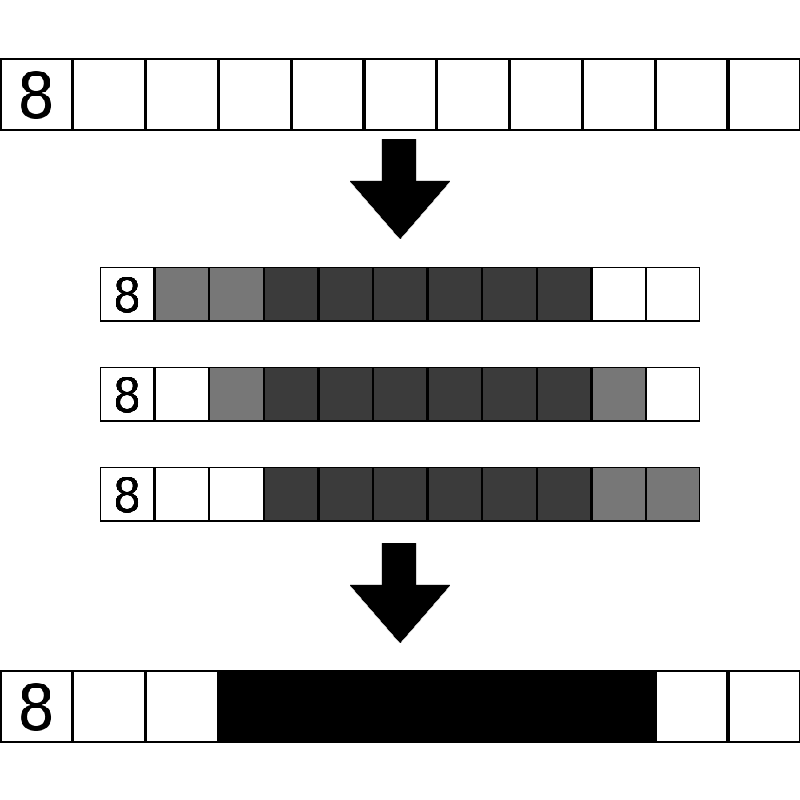
\includegraphics[width=\textwidth]{images/elimination_solver_example_a.png}
        \caption{pola wspólne dla wszystkich kombinacji zostają naniesione na planszę}
    \end{subfigure}
    \hspace{0.1\textwidth}
    \begin{subfigure}[b]{0.35\textwidth}
        \centering
        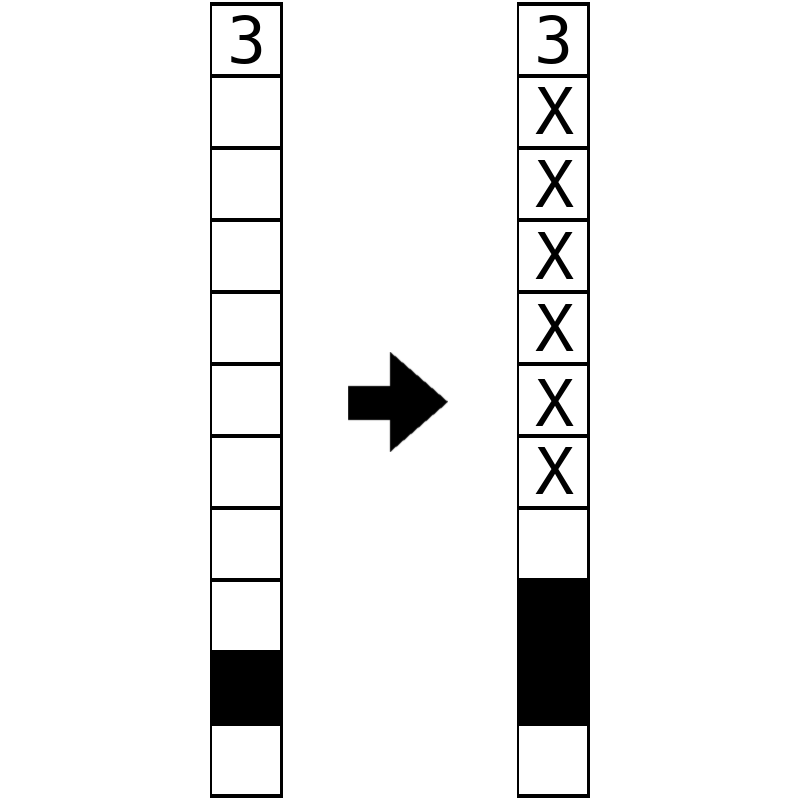
\includegraphics[width=\textwidth]{images/elimination_solver_example_b.png}
        \caption{korzystając z informacji z wiersza, solver wnioskuje stan większości pól w kolumnie
        (x oznacza pole definitywnie puste)}
    \end{subfigure}
    \caption{Przykład wnioskowania na podstawie możliwych kombinacji}
\end{figure}

    Solver zaczyna od pustej planszy. Na początku generowane są wszystkie kombinacje dla każdej z
linii, a linie wrzucane są do kolejki \textit{last-in first-out}. Następnie solver przechodzi do
rozwiązywania. Dopóki kolejka nie jest pusta, to są linie, których komibnacje należy zweryfikować.
Z kolejki usuwana jest sprawdzana linia. Dla tej linii następują dwa kroki: najpierw, eliminowane
są kombinacje sprzeczne z układem danej linii. W wypadku tego solvera, każda komórka znajduje się
w jednym z trzech stanów: \textit{pełny}, \textit{pusty} i \textit{nieznany}. Stan \textit{nieznany}
komórki dopuszcza kombinacje zawierające komórkę pełną lub pustą; pozostałe stany wymagają
zgodności stanu ze stanem komórki w kombinacji. Po eliminacji sprzecznych kombinacji, dochodzi
do porównania kombinacji. Jeśli istnieje komórka w linii, której stan jest \textit{nieznany}, a
wszystkie pozostałe kombinacje mają ustawiony dla niej ten sam stan, to stan komórki jest aktualizowany,
a prostopadła linia zostaje dodana do kolejki do weryfikacji (następuje przy tym upewnienie, że
w kolejce nie ma powtórzeń). Kiedy kolejka zostanie opróżniona, sprawdzane są linie.
Jeśli wszystkie linie mają jeden możliwy stan, to znaczy że zostało znalezione rozwiązanie. Jeśli
któraś z linii nie ma możliwej kombinacji, to nie istnieje rozwiązanie przy dokonanych założeniach.
W przeciwnym wypadku, solver zakłada poprawność jednej z kombinacji dla linii
o kilku możliwych kombinacjach. Jako że wskutek założenia stan linii zmienił się, to do kolejki
dodawane są linie prostopadłe. Następnie wywoływana jest w sposób rekursyjny metoda rozwiązująca
nonogram dla obecnego stanu planszy. Jeśli rozwiązanie nie zostanie znalezione w tej gałęzi, to
solver zakłada poprawność kolejnej kombinacji dla tej linii.

\begin{pseudokod}[H]
    %\SetAlTitleFnt{small}
    \SetArgSty{normalfont}
    \SetKwFunction{SprawdzLinie}{SprawdzLinie}
    \SetKwFunction{NalozKombinacje}{NalozKombinacje}
    \SetKwFunction{UzupelnijKolejke}{UzupelnijKolejke}
    \KwIn{Lista wierszy $R$ i kolumn $C$, kolejka $Q$}
    \KwOut{Czy znaleziono rozwiązanie \texttt{true/false}}
    \ForEach{$linia \in Q$}{
        \SprawdzLinie{$linia$}\;
    }
    \If{$(\forall linia \in R \bigcup C)(|linia.kombinacje| = 1)$}{
        \texttt{return true}\;
    }
    \uElseIf{$(\exists linia \in R \bigcup C)(|linia.kombinacje| = 0)$}{
        \texttt{return false}\;
    }
    \Else{
        $zakladanaLinia \leftarrow$ pierwsza linia z wieloma kombinacjami\;
        \ForEach{$komb \in zakladanaLinia.kombinacje$}{
            $kopiaR \leftarrow kopiuj(R)$\;
            $kopiaC \leftarrow kopiuj(C)$\;
            \NalozKombinacje{$zakladanaLinia, komb$}\;
            \UzupelnijKolejke{$Q$}\;
            \If{\texttt{SolverEliminacyjny}($kopiaR, kopiaC, Q$)}{
                $R \leftarrow kopiaR$\;
                $C \leftarrow kopiaC$\;
                \texttt{return true}\;
            }
        }
        \texttt{return false}\;
    }
    \caption{SolverEliminacyjny}\label{alg:eliminationSolver}
\end{pseudokod}

    Istotna uwaga dotyczy charakterystyki wierszy i kolumn. W celu umożliwienia działania procedury
został wykorzystany mechanizm obecny w wielu powszechnie używanych językach programowania, mianowicie
mechanizm płytkiej kopii. Mimo że listy wierszy i kolumn zawierają inne obiekty (listy), to obiekty
komórek przechowywane w tych zagnieżdżonych listach są takie same. Dzięki temu, modyfikując stan
komórki w liście wierszy w $n$-tym wierszu i $m$-tej komórce, modyfikujemy także stan komórki
zawartej w $n$-tej komórce w $m$-tej kolumnie w liście kolumn.
